\section{Background}

As noted in Chapter \ref{chapter:prelude}, protein-protein
interactions from single organisms have been organized into networks,
where proteins are nodes and network edges represent interactions
between proteins \cite{han04}. These protein-protein interaction (PPI)
networks have two types of nodes, hubs and non-hubs
\cite{barabási2004network}. Characterizing protein nodes in this
manner happened after PPI networks were observed to be scale-free,
i.e.\, the distribution of the number of proteins each network protein
interacts with follows a power law where a small percentage of network
proteins have the majority of interactions in the network
\cite{jeong2001lethality}. These highly connected network proteins are
referred to as network hubs. Although the scale-freeness of networks
has been debated
\cite{han2005effect,rachlin2006biological,stumpf2005subnets}, the
property indicates that networks are robust to perturbations on random
nodes because most nodes are not hubs
\cite{albert2000error,li2006protein}, and the specific removal of hub
nodes can drastically alter network structure by removing many
interactions \cite{albert2000error,li2006protein}.

The study of host network hubs in virus-host systems biology is
important for two reasons. First, HCV, HIV, influenza virus,
Epstein-Barr virus, and other human viruses preferentially interact
with hubs in the human PPI network
\cite{calderwood07,dyer08,dechassey08,tastan09}. It has been
speculated that this viral targeting of host hubs is an efficient way
to rewire the host network \cite{calderwood07}. Second, host hubs are
important for the study of virus interactions with host networks
because they have been well studied, and have a number of important
properties that could explain virus-host interactions. Knowledge of
host hub properties from network systems biology provides a number of
host protein features that might be targeted by viruses.

Most of what has been learned about host hubs is useful to consider
when looking for properties of virus targeted host proteins. Hubs are
evolutionarily conserved \cite{fraser2002evolutionary}. When compared
across organisms, hubs have lower mutation rates than other network
proteins \cite{batada2006evolutionary}. Furthermore, comparing the
number of interactions for hub proteins across human, fly, worm, and
yeast revealed that hub proteins have similar numbers of interactions
across all organisms \cite{fox09}. Studies of high quality PPI
networks have revealed a correlation between the number of PPIs a
protein participates in and its importance to the cell
\cite{he2006hubs}. This has led to the conclusion that hubs are
essential for cell survival \cite{han04,batada2006evolutionary}. Hubs
also have only small changes in gene expression across different
conditions as compared to other network proteins \cite{lu2007hubs}.
Proteins mutated in cancer are more likely to be network hubs
\cite{jonsson2006global}. Finally, hubs allow for network
evolution. Gene duplications are observed more often for hub proteins,
creating redundancy in the PPI network that can lead to
neofunctionalization
\cite{kafri2008preferential,teshima2008neofunctionalization}.

\subsection{Intermodular and intramodular hubs}

Since the study of hubs is important to the study of networks, or
interactomes, hubs have been investigated further, and it has been
revealed that they can be divided into two classes, or modes, by
examining their co-expression with their interactome neighbors
\cite{taylor09}. In human, hubs are classified as intermodular or
intramodular. Intermodular hubs are defined as being co-expressed with
their neighbors in certain tissues, while intramodular hubs are
characterized by co-expression with their neighbors in most tissues
\cite{taylor09}. This hub distinction based on gene co-expression is
important for cancer. It has been demonstrated that the change between
intermodular and intramodular modes is predictive of breast cancer
patient survival \cite{taylor09}.

The case for hub modularity was first made in yeast, where hubs were
classified as `date' or `party' using time series expression data to
look at the co-expression of hubs and the proteins they were observed
to bind to in the yeast interactome \cite{han04}. The distribution of
hub interactome neighbor co-expression values was observed to have two
modes. Hubs in the party hub mode were described as having a higher
level of interactome neighbor co-expression than hubs in the date hub
mode. Non-hub proteins did not show this bimodal distribution of hub
and neighbor co-expression. Further analysis revealed that date hubs
served as connections between protein modules and complexes, while
party hubs acted as their central components \cite{fraser05}. This
observation led to the rebranding of date and party hubs as
intermodular and intramodular hubs, respectively. Taylor et
al.\ extended these terms to include human hubs, demonstrating that
intermodular hubs were co-expressed with their neighbors in specific
tissues, while intramodular hubs showed neighbor co-expression across
most tissues \cite{taylor09}. These hub classifications have been
debated for both yeast and human. In yeast, the analysis of larger
interactome datasets failed to replicate the hub distinction
\cite{batada06,batada07}. In human, using a more controlled
normalization of the expression data used by Taylor et al.\ caused the
hub class distinction to disappear \cite{agarwal09}. Specifically, the
GCRMA algorithm \cite{wu2004model}, which controls for probe affinity,
was used instead of the Affymetrix MAS5 algorithm
\cite{hubbell2002robust} adopted by Taylor et al..

Intermodular and intramodular hubs have specific properties in both
yeast and human \cite{taylor09,fraser05}. Intermodular hubs provide
temporally and spatially constricted connections between intramodular
hubs, which serve as components of cell machinery \cite{fraser05}.
These connections allow intermodular hubs to direct macromolecular
complexes in a time and space dependent manner. These intermodular hub
proteins have been found to be larger than intramodular hub proteins,
and have more unique domains and peptide binding motifs than
intramodular hubs \cite{taylor09}. Intramodular hubs have been found
to share more molecular functions with their PPI neighbors than
intermodular hubs \cite{taylor09}. As expected of hubs that modulate
cellular activity, intermodular hubs were found to be enriched in cell
signaling domains \cite{taylor09}. In yeast, intermodular hubs are
more disordered, or less structured, than intermodular hubs
\cite{ekman2006properties,singh2007role}. This is consistent with the
observation that intermodular hubs have few binding surfaces, while
intramodular hubs have multiple, similar binding regions that allow
many interactions to occur at once \cite{kim2008role}. Note that this
is not inconsistent with the finding that human intermodular hubs have
more unique binding regions than intramodular hubs. In fact, human
intramodular hubs were found to have greater globularity, or domain
coverage, than intermodular hubs \cite{taylor09}, which is consistent
with the yeast hub result that intramodular hubs have more protein
binding regions. Intramodular hubs have also been found to have lower
evolutionary rates than intermodular hubs
\cite{fraser2005modularity}. This may be caused by the greater
globularity and more structured regions in intramodular hubs as
compared to intermodular ones \cite{kahali2009exploring}.

In this chapter we provide new evidence for the inter/intramodular hub
distinction, and ask if hub proteins that interact with virus proteins
favor one hub type over the other. The work presented here is
important for two reasons. First, it contributes to the network
biology field by reaffirming the existence of two hub classes by
showing that viruses prefer one hub class over another. Second, it
aids the study of virus-host networks by refining the observation that
viruses preferentially interact with hub proteins. This refinement
focuses the multiple hub properties that might be behind the virus
preference into a few testable hypotheses for future studies.

%% Then I can say that we can leverage all of these findings if we can
%% show a hub preference. Showing that viruses prefer one hub type over
%% another will give us a set of properties to test to see what viruses
%% like. This will give us a set of properties that we can test; open up
%% a list of testable hypothesis with one study.

%% Why not test virus proteins individually for these properties? This
%% gives you a reason to have the hypothesis, some justification for the
%% study. These properties are important because they give us a better
%% understanding of the integrations between virus and host. This is the
%% best way to go.

\section{Results}

\begin{figure}
\begin{center}
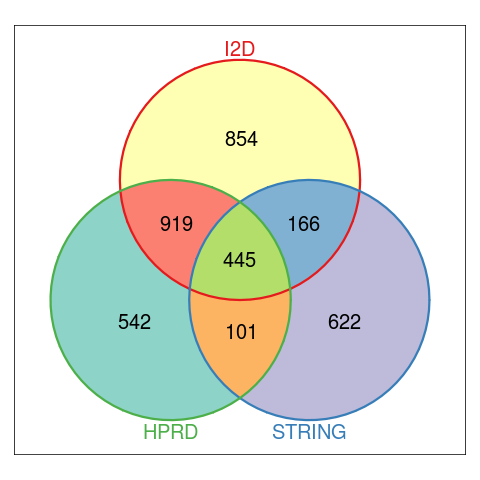
\includegraphics[scale=0.5]{figs/hubs_overlap}
\end{center}
\caption[Comparing hubs across human interactomes]{\small In this
  study we used three human networks, I2D, STRING, and HPRD. To find
  hubs for each network, we took the top 20\% most connected
  nodes. Each network had a different hub set due to differing network
  size and connectivity. Here we show the overlap between hub sets for
  the three networks. \label{fig:sysBio:hubOverlap}}
\end{figure}

\subsection{Hub classification}

In this study, we reexamined the hub class hypothesis in human with
the goal of investigating virus hub preference. We adopted the same
approach used by Taylor et al., but substituted their expression
dataset with one from COXPRESdb \cite{obayashi07}, which is larger in
terms of genes and samples. To ensure that our results were robust to
interactome changes, we used three separate human interactomes from
the Interologous Interaction Database (I2D) \cite{brown05}, the Search
Tool for the Retrieval of Interacting Genes/proteins (STRING)
\cite{von07}, and the Human Protein Reaction Database (HPRD)
\cite{prasad08}. I2D, with roughly 150 thousand edges connecting 11.5
thousand proteins, is the largest network, but it also contains the
most interaction predictions. HPRD has around 35 thousand edges
between nine thousand proteins. This network has high quality
interactions curated from the literature. Like I2D, STRING has many
predicted interactions to complement interactions from the literature,
resulting in a network of about 140 thousand interactions between six
thousand proteins. For each network, we designated the 20\% most
connected proteins as hubs \cite{bertin07}. Due to connectivity
differences, each interactome resulted in a different set of hubs
(Figure \ref{fig:sysBio:hubOverlap}). To make the hub classifications
for each network, we used Pearson correlation coefficients (PCCs) from
COXPRESdb to indicate correlated gene expression between hub proteins
and their neighbors, and obtained an average PCC for each hub by
averaging the PCCs of the hub's neighbors \cite{han04,taylor09}. We
refer to the distribution of average PCC values for hubs as dPCC. For
each interactome's dPCC, we used a likelihood ratio test
\cite{ertel08} to confirm that a bimodal distribution was a
significantly better fit for the data than a unimodal
distribution. The resulting bimodal distributions for each network did
not allow an easy separation between inter/intramodular hubs because
of the large overlap between the two modes, so we fit a mixture of two
Gaussian distributions to binned versions of each network's dPCC
(Figure \ref{fig:sysBio:fig1}a). We found that limiting hubs in one
network to those present in one or both of the other two networks
resulted in a stronger bimodal signal for each dPCC (Figure
\ref{fig:sysBio:fig1}b). For the remainder of the study, we limited
hubs in one network to only proteins classified as hubs in one of the
other two networks.

\begin{figure}
\begin{center}
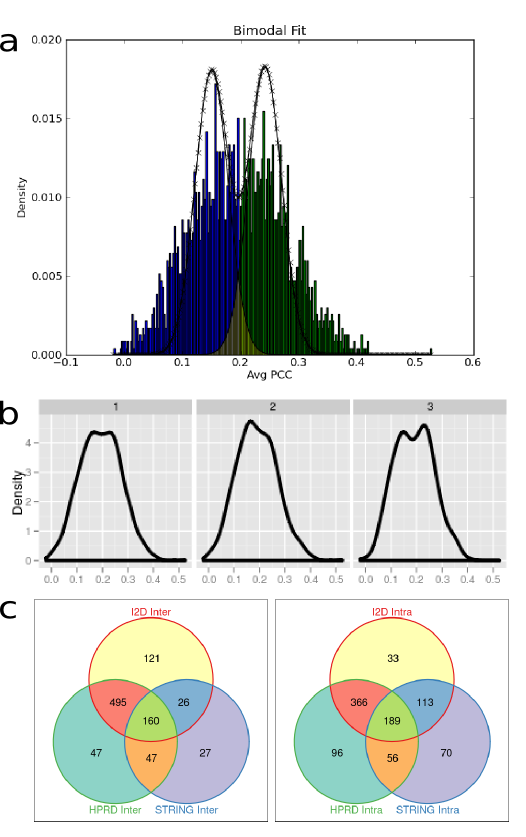
\includegraphics[scale=0.9]{figs/sysBio_1}
\end{center}
\caption[Establishing inter/intramodular hubs]{\small This figure
  illustrates how we have classified intermodular and intramodular
  hubs. (a) The distribution of hub average PCC values (dPCC) for I2D
  hubs was fit with a bimodal distribution. Hubs were assigned to
  either the intermodular mode (blue) or intramodular mode (green) of
  the bimodal distribution. (b) The dPCC each for network hubs became
  more bimodal as the number of interactomes the hub had to be present
  in increased. The density curves shown here for the I2D interactome
  are for all hubs present in I2D (1), hubs in I2D and STRING or HPRD
  (2), and hubs present in all three interactomes (3). (c)
  Inter/intramodular hub classifications were compared for I2D,
  STRING, and HPRD. In an effort to make are results robust to network
  changes, we focused on hubs with the same classification in at least
  two networks. \label{fig:sysBio:fig1}}
\end{figure}

We obtained intermodular and intramodular hub sets for each
interactome by assigning hubs to the most likely mode of the
interactome's dPCC. As defined before, intramodular hubs in the higher
mode were co-expressed with their neighbors in most tissues, while
intermodular hubs in the lower mode were co-expressed with their
neighbors in certain tissues. Like the hub, non-hub classification,
interactomes differed in their inter/intramodular hub sets, but there
was much overlap despite the networks having different connectivities
(Figure \ref{fig:sysBio:fig1}c). Final hub classifications were
determined by the most frequently observed hub class across the three
networks. Hubs that were only present in two interactomes, and had
conflicting class assignments, were not considered in the study. Hub
classifications were stochastic because of equally likely hub
assignments, making hub class assignments differ slightly between
runs, but our results were qualitatively similar for all runs. Here we
present the results for one run.

\subsection{Hub class properties}

Using hubs with consistent inter/intramodular classifications in at
least two networks, we examined biological features of intermodular
and intramodular hubs. As reported by Taylor et al., intermodular hubs
had more linear motifs \cite{puntervoll03} per residue and more unique
SMART domains \cite{letunic2008smart} per protein than intramodular
hubs (one-tailed Wilcoxon tests, p-value $<$ 0.03 for both). Taylor et
al.\ also reported that intramodular hubs were longer than
intermodular hubs, but we found no difference in protein length
between the hub classes. We used DAVID \cite{dennis03} to find KEGG
pathways \cite{kanehisa08} and Gene Ontology \cite{ashburner00} terms
enriched in each hub class compared to all hubs. Intermodular hubs
were enriched in genes involved in signal transduction, kinase
cascades, anatomical structure morphogenesis and development, cellular
development, and multicellular organismal development
(Bonferroni-corrected p-value $<$ 0.01). Intramodular hubs were
enriched in genes annotated with translation, mRNA metabolic process,
RNA splicing, ribosome and proteasome components, nucleotide binding,
pyrophosphatase activity, and cell cycle (Bonferroni-corrected p-value
$<$ 0.01). These hub enriched terms are consistent with what has been
reported for hubs in both yeast and human \cite{taylor09,fraser05}.

\subsection{Virus hub preference}

With our hub classes established, we gathered three sets of virus-host
interactions to test for an association between hub class and hub
proteins that interact with virus proteins. We found human proteins
that interacted with an HIV protein by combining VirusMINT
\cite{chatr08} and the NCBI HIV-1, Human Protein Interaction Database
\cite{fu09}. For HCV, we relied on a collection of virus-host
interactions identified by yeast two-hybrid screens and a literature
search \cite{dechassey08}. For influenza virus, we used curated
interactions gathered to study influenza virus replication
\cite{konig2009human}.

\begin{table}\footnotesize
\begin{center}
\begin{tabular}{|l|c|c|c|}
\hline
\multicolumn{4}{|c|}{Average hub-neighbor co-expression}\\
\hline
Virus & Intermodular & Intramodular & P-value \\
\hline
HCV &        73/655 &  56/668 &  0.948350202594 \\
HIV &       93/635 & 130/594& 0.00380164624435 \\
Influenza & 40/688 & 88/636 &  4.77173152977e-06 \\
\hline
\hline
\multicolumn{4}{|c|}{Median hub-neighbor co-expression}\\
\hline
Virus & Intermodular & Intramodular & P-value \\
\hline
HCV &        71/646  & 52/646  & 0.958559296013\\
HIV & 95/622  & 121/577 & 0.01952745875\\
Influenza & 39/678  & 84/614  & 6.9130570599e-06\\
\hline
  \end{tabular}
\end{center}
\caption[Fisher's test for virus hub preference]{\small The table
  shows the number of virus targeted inter/intramodular hubs
  considered when testing for an association between hub class and
  virus interaction, as well as the results from a one-tailed Fisher's
  exact test. HIV and the influenza virus target proteins that are
  enriched in intramodular hubs, while HCV targeted proteins almost
  show a preference for intermodular hubs. Calculations were performed
  using the average and median to calculate a measure of co-expression
  between hubs and their interacting neighbors (see
  text). \label{tbl:sysBio:bindingFisher}}
\end{table}


\begin{figure}
\begin{center}
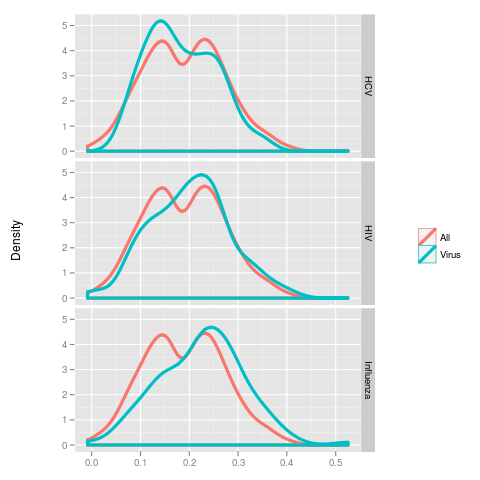
\includegraphics[scale=0.5]{figs/sysBio_2_new}
\end{center}
\caption[Virus hub preference]{\small This figure visually compares
  the virus hub preference for HCV, HIV, and influenza virus. For each
  virus, dPCC density curves for virus targeted hubs were plotted
  against the dPCC density curve for all intermodular and intramodular
  hubs in the human I2D network. We used only hubs present in I2D and
  another human network. Hubs that interacted with HIV or influenza
  virus preferred the intramodular mode of the dPCC bimodal
  distribution. \label{fig:sysBio:fig2}}
\end{figure}

In an attempt to detect a trend for virus-host interactions, we
separately tested hub sets targeted by HCV, HIV, and influenza virus
for an inter/intramodular hub class preference using a one-tailed
Fisher's exact test (Table \ref{tbl:sysBio:bindingFisher}). HIV and
influenza targeted hubs tended to be intramodular (Figure
\ref{fig:sysBio:fig2}). On the other hand, HCV targeted hubs were
almost significantly associated with intermodular hubs (Fisher's exact
test, p-value $<$ 0.055).

%% We next checked to see if the HIV
%% intramodular preference held for the three individual
%% interactomes. For each interactome, we classified all hubs based on
%% the network's dPCC, and found that HIV preferred intramodular hubs
%% over intermodular hubs in each case (p-value $<$ 0.02). There were
%% not enough experimental interactions for HCV to make a hub preference
%% conclusion for individual interactomes. Using a combination of
%% predicted and experimentally determined HCV targeted proteins, we
%% found that HCV showed an intramodular hub preference only for the HPRD
%% interactome (p-value $<$ 0.03).

To further study the viruses, we turned to small interfering RNA
(siRNA) screens for virus dependency factors (VDFs)
\cite{bushman09,yeung09,Li09,konig2009human}. In these screens, host
genes were knocked down in virus infected cells, and the effect on the
virus is observed. Genes whose expression depletion negatively
affected the virus were recorded as VDF hits, i.e.\, host factors that
are required by the virus \cite{bushman09}. For HIV, we merged results
from four siRNA screens that searched for VDFs required for HIV
replication \cite{bushman09,yeung09}. These datasets of had few genes
in common, but genes across datasets often had roles in the same
pathways \cite{yeung09}. HCV siRNA results were taken from several
screens that covered the full HCV life cycle \cite{Li09}. Influenza
virus screen results were taken from a study of VDFs involved in
influenza replication \cite{konig2009human}. Just as host proteins
found to bind to virus proteins were enriched in hubs, we found that
VDFs had more interactome neighbors than genes with no virus
association (one-sided Wilcoxon test, HCV: p-value $<$ 6e-8, HIV:
p-value $<$ 3e-11, influenza: p-value $<$ 9e-19). Using Fisher's exact
test again, we found that HIV still showed an intramodular hub
preference for the siRNA data, while HCV and the influenza virus did
not (Table \ref{tbl:sysBio:rnaiFisher}).

The bimodality of each network's dPCC might have been caused by a
significant difference between hub classes in terms of the number of
interacting neighbors, or degree, considered for each hub,
i.e.\ proteins in one hub class would have significantly different
numbers of interaction neighbors than proteins in the other hub class
\cite{taylor09}. Taylor et al.\ addressed this concern and found no
difference in the degree distributions of the hub classes
\cite{taylor09}. We compared intermodular and intramodular hub degree
distributions for each network separately using a one-tailed Wilcoxon
test. For the I2D and STRING interactomes, we found that intramodular
hubs had more neighbors than intermodular hubs (p-value $<$ 3.5e-12
and p-value $<$ 5.5e-12, respectively). For HPRD, neither hub class
had more interactions. Since we found a degree distribution difference
between inter/intramodular hubs for the I2D and STRING networks, we
repeated the classification of host hub proteins using the median
instead of the average when summarizing hub neighbor co-expression. If
the degree difference between inter/intramodular hubs was causing the
hub distinction, using the median instead of the average would solve
this problem by removing the influence of outliers in a hub's
collection of neighbor co-expression correlations, and controlling for
hub degree. Using the median instead of the average did not produce
qualitatively different results for virus-host protein interactions
(Table \ref{tbl:sysBio:bindingFisher}). For the siRNA data, the
association between HCV host dependency factors and intramodular hubs
became significant (Table \ref{tbl:sysBio:rnaiFisher}).

\begin{table}\footnotesize
\begin{center}
\begin{tabular}{|l|c|c|c|}
\hline
\multicolumn{4}{|c|}{Average hub-neighbor co-expression}\\
\hline
Virus & Intermodular & Intramodular & P-value \\
\hline
HCV &  25/703 & 38/686 & 0.0581221952106       \\
HIV &   58/670 &  106/618 & 3.79707703564e-05    \\
Influenza & 34/694 & 36/688&  0.441928925248 \\
\hline
\hline
\multicolumn{4}{|c|}{Median hub-neighbor co-expression}\\
\hline
Virus & Intermodular & Intramodular & P-value \\
\hline
HCV &   21/696  & 41/657  & 0.00477984148923   \\ 
HIV & 56/661  & 106/592 & 8.58550353701e-06\\
Influenza & 36/681  & 34/664  & 0.599420611669\\
\hline
  \end{tabular}
\end{center}
\caption[Fisher's test for virus hub host factor preference]{\small
  The table shows the number of inter/intramodular hubs considered
  when testing for an association between hub class and virus host
  factors, as well as the results from a one-tailed Fisher's exact
  test. Only host factors required for HIV replication are associated
  with intramodular hubs. Calculations were performed using the
  average and median to calculate a measure of co-expression between
  hubs and their interacting neighbors (see
  text). \label{tbl:sysBio:rnaiFisher}}
\end{table}


For each virus, we intersected siRNA screen hits with host proteins
that interacted with virus proteins to arrive at virus-host protein
binding interactions that might play an important role in the virus
life cycle. Figure \ref{fig:sysBio:fig3} shows the network of
connections between of these virus targeted inter/intramodular hubs
and virus proteins. Human hubs were placed into functional categories
according to the literature \cite{bushman09,taylor09}. HIV targeted
intramodular hubs included proteins involved with transcription and
splicing, nuclear transport, HIV cell entry and budding, and the
proteasome. The four intramodular HCV targeted hubs were
serine/threonine-protein kinase TBK1, actin-modulating protein CFL1,
nuclear import protein IPO5, and CDK6. Differing from HCV and HIV
targeted intramodular hubs, some influenza virus targeted intramodular
hubs were involved in apoptosis and the cell cycle. Intermodular HCV
targeted hubs included proteins involved in transcription,
translation, and cellular transport. Intermodular hubs found to
interact with all three viruses included members of the Jak/STAT and
MAPK signaling pathways.

\begin{figure}
\begin{center}
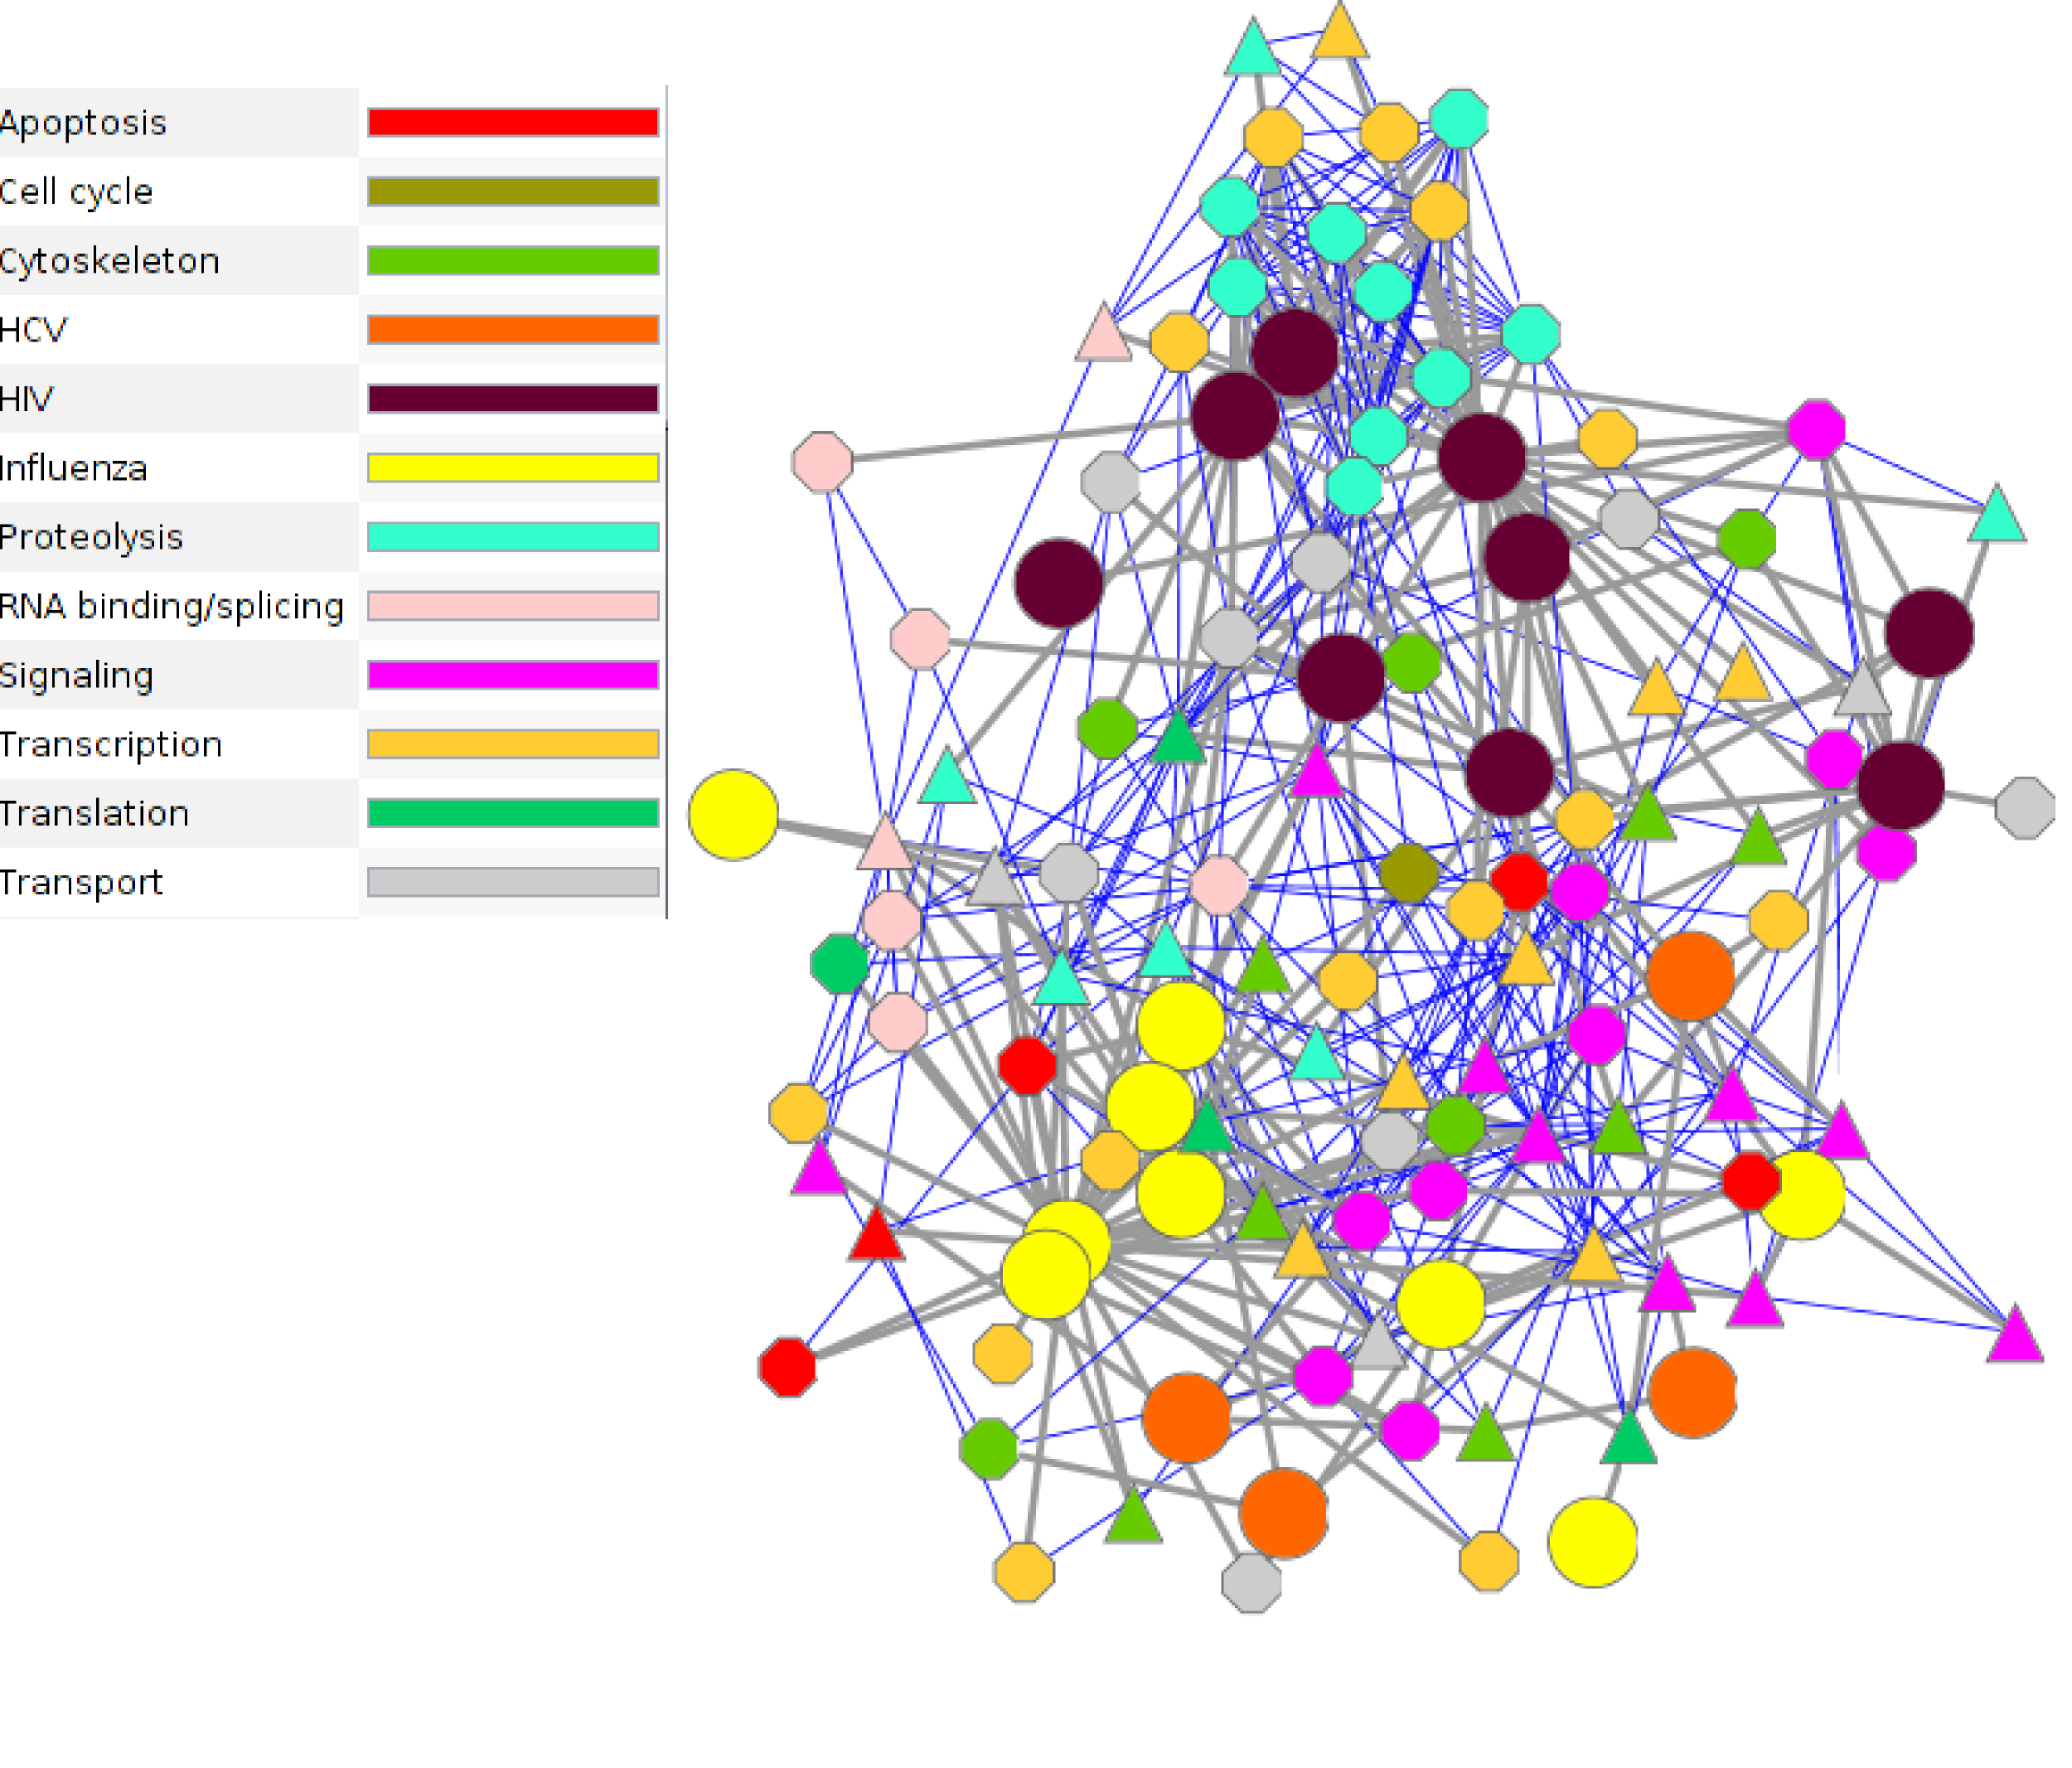
\includegraphics[scale=0.7]{figs/sysBio_3}
\end{center}
\caption[Virus-host hub network]{\small Here we show the
  inter/intramodular hubs targeted by HCV, HIV, and the influenza
  virus. Virus proteins are large circles. Intermodular hubs are
  triangles, and intramodular hubs are octagons. Virus-host
  interactions are thick lines, while human-human interactions are
  thin and blue. Human hubs are colored by biological
  function. \label{fig:sysBio:fig3}}
\end{figure}

\section{Discussion}

To find a biological reason for the hub preference observed for HIV
and influenza virus, we focused on the roles of human protein
complexes in virus life cycles. HCV, HIV, and influenza virus all
encode less than 20 proteins, and must rely on human proteins to
accomplish virus replication \cite{Li09,tastan09}. There is much
anecdotal evidence that HIV proteins interact with human complexes to
accomplish important roles in HIV replication \cite{bushman09}. HIV
proteins interact with the mediator, P-TEFb, and elongin complexes to
accomplish HIV transcription. HIV splicing is directed by HIV proteins
interacting with hnRNP complexes. Interactions of HIV proteins with
the chaperone containing TCP1 complex might play a role in HIV
budding. For HCV infection, the role of human complexes is less
clear. An siRNA screen indicated that the Golgi-associated retrograde
transport complex might play a role in HCV replication
\cite{Li09}. Influenza virus has been predicted to interact with host
complexes such as the ribosome, proteasome, and splicesome
\cite{konig2009human}. To establish a link between human protein
complexes and viruses, we counted the number of complexes a human
protein participated in using complexes listed in HPRD. In our hub set
for HPRD, more than half of the hubs participated in at least one
complex, which was significantly more than the fraction of complexed
proteins found in the entire network (p-value $<$ 9e-57). For each of
the three viruses, we used a one-tailed Wilcoxon test to show that
virus targeted human proteins participated in more protein complexes
than other human proteins (HIV: p-value $<$ 0.002, HCV: p-value $<$
0.02, influenza: p-value $<$ 6e-4). This is expected from the
observation that host hub proteins participate in more complexes than
other network proteins, so we conducted a further test with HIV that
revealed that virus targeted hub proteins participated in more
complexes than other hub proteins (one-sided Fisher's exact test,
p-value $<$ 0.03).

In yeast, intermodular hubs connect modules and complexes, while
intramodular hubs serve as their central components
\cite{fraser05}. Using protein complexes described in HPRD, we
confirmed that human intramodular hubs participated in more complexes
than intermodular hubs (one-sided Wilcoxon test, p-value $<$ 0.02). If
viruses must modulate the activity of protein complexes, they could do
so by interacting with complexes directly through intramodular hubs,
or they could interact with proteins that form connections between
complexes, the intermodular hubs. Given that HIV and influenza virus
prefer to interact with human proteins involved in many complexes, and
intramodular hubs are involved in more complexes than intermodular
hubs, we propose that some virus proteins interact preferentially with
intramodular hubs because they are involved in more protein complexes
than intermodular hubs.

\section{Conclusion}

Our results have further demonstrated the distinction between
intermodular and intramodular hubs. We found that by considering hubs
present in multiple networks, this distinction becomes more evident.
We used this observation to classify human hubs that have direct
protein interactions with virus proteins, and found that HIV and
influenza virus targeted hubs were more likely to be intramodular than
intermodular. HCV targeted proteins did not show a significant hub
type preference, but since the siRNA data did show an intramodular
preference, this may change as more interactions are
gathered. Compared to intramodular hubs, intermodular hubs had more
linear motifs per residue and more unique SMART domains. Intermodular
hubs were enriched in signaling and developmental pathways while
intramodular hubs were enriched in translation and mRNA
processing. Intramodular hubs participated in more protein complexes
than intermodular hubs, and, given that HIV and influenza virus
proteins prefer to interact with members of many complexes, this bias
might be causing the hub class preference.

Knowing that some viruses have an intramodular hub preference aids the
study of virus proteins in two ways. First, a virus intramodular hub
preference is beneficial for virus-host network studies that are
functionally annotating virus proteins based on their host binding
partners. In single organisms networks, proteins that interact with
each other are often in the same cellular pathways, and share the same
functions \cite{segal2003discovering}. This observation has been used
to annotate proteins with unknown function with the functions of
proteins with which they interact
\cite{karaoz2004whole,sharan2007network}. This annotation method has
been extended to virus-host networks, annotating virus proteins based
on the functions of their interacting host proteins
\cite{calderwood07}. Since intramodular hubs are more likely to be
functionally similar to the proteins they interact with
\cite{taylor09}, the virus intramodular hub preference justifies
annotating virus proteins using virus-host networks, while an
intermodular hub preference would cast doubt on this annotation
method.

The second way that a virus intramodular hub preference aids the study
of virus proteins is by providing protein features that viruses might
be targeting when they interact with host proteins. Here we provided
evidence that virus proteins prefer to interact with intramodular hubs
because they participate in host protein complexes more often than
intermodular hubs. Intramodular hub proteins are also more structured
than intermodular hubs, participate in more cellular housekeeping
activities than intermodular hubs, and evolve at lower rates than
intermodular hubs. Further study is needed to see if these features
might also be targeted by virus proteins, and to determine the
importance of each feature to viruses.

\section{Methods}
  \subsection{Human interactome}
    We converted the human I2D (accessed October 2009), human STRING
    (version 8.2), and HPRD (release 8) interactomes to networks of
    Entrez Gene IDs using ID mapping provided by UniProt
    \cite{citeulike:6008733}, gProfiler \cite{reimand2007g}, and
    NCBI's eutils. Network hubs were found for each interactome
    separately by locating the lowest degree in the top 20\% of
    connected genes, and taking all genes with at least this
    degree. Bimodal curves for each interactome's hub average PCC
    distribution were found using gradient descent to minimize the
    log-likelihood of a binned distribution. The number of bins for
    each distribution was determined by dividing the total number of
    data points by a bin divisor. For individual networks, we used a
    bin divisor of 11 for I2D and 10 for STRING and HPRD. For
    distributions made using hubs present in at least two networks, we
    fit a bimodal curve using a bin divisor of 6 for STRING and 9 for
    I2D and HPRD.

  \subsection{Virus-host interactomes}
    We gathered HIV-human protein interactions from NCBI and
    VirusMINT. Both virus-host interaction datasets label interactions
    by type. We focused on interaction types describing direct protein
    interactions, or modifications. We used VirusMINT interactions
    labeled with MINT interaction IDs 0006 (anti bait
    coimmunoprecipitation), 0007 (anti tag coimmunoprecipitation),
    0018 (two hybrid), 0019 (coimmunoprecipitation), 0027
    (cosedimentation), 0045 (experimental interaction detection), 0096
    (pull down), 0416 (fluorescence microscopy), 0424 (protein kinase
    assay), 0435 (protease assay), 0515 (methyltransferase assay),
    0889 (acetylation assay). For the NCBI database, we used
    acetylated by, acetylates, binds, cleaved by, cleaves, degraded
    by, degrades, dephosphorylates, methylated by, myristoylated by,
    phosphorylated by, phosphorylates, ubiquitinated by edges. We
    gathered HIV siRNA results from two sources covering four studies,
    and converted these hits to Entrez Gene IDs. Three studies were
    summarized in Table 4 of the supplementary document supplied by
    Bushman et al.\ at http://www.hostpathogen.org
    \cite{bushman09}. The fourth study was taken from Figure S2 in an
    article by Yeung et al. \cite{yeung09}.

    HCV-human protein interactions were taken from de Chassey et
    al. \cite{dechassey08}. HCV siRNA results were taken as genes that
    showed a decrease in infection, listed in supplementary material
    SD1 and SD2 columns B-E \cite{Li09}.

    Influenza-human protein interactions and siRNA hits were taken
    from a study of host factors involved in influenza replication
    \cite{konig2009human}. For the protein interactions, we ignored
    interactions where no virus protein was specified.

   \subsection{Peptide motif and SMART domain annotations}
    Protein sequences form three human interactomes, I2D, STRING, and
    HPRD, were scanned for peptide motifs and SMART domains. Protein
    sequences for the STRING and HPRD interactomes were taken from
    their respective databases. Protein sequences for the I2D network
    were taken from UniProt. Human proteins were scanned for SMART
    domains using batch access. Human proteins were annotated with the
    136 peptide motifs described in the ELM Resource by downloading
    regular expressions for each motif from the resource, and matching
    them against all human protein sequences. The networks used in
    this study were composed of Entrez Gene IDs, and multiple proteins
    may correspond to one Entrez Gene ID. For peptide motif and SMART
    domain annotations for each Entrez Gene ID, we averaged the
    annotations of all the proteins for which it coded.

  %% \subsection{HCV-human interaction predictions}
  %%   Multiple alignments for HCV proteins F, CORE, E1, E2, NS2, NS3,
  %%   NS4A, NS4B, NS5A, NS5B, and P7 were obtained from the Los Alamos
  %%   National Laboratory HCV sequence database
  %%   (http://hcv.lanl.gov/content/sequence/NEWALIGN/align.html). HCV
  %%   proteins were annotated with 136 ELMs using regular
  %%   expressions. For each of the 53 ELMs found to be conserved on at
  %%   least 90\% of an HCV protein's alignment, we found either a
  %%   PROSITE domain \cite{hulo08} known to interact with the ELM, or a
  %%   set of proteins known to interact with the ELM \cite{evans09}. We
  %%   used the ELM Resource and ScanProsite to annotate proteins from
  %%   I2D, STRING, and HPRD. Predictions were made using the method
  %%   described by Evans et al. \cite{evans09}.

%ScanProsite \cite{decastro06}

